\documentclass[12pt]{ctexart}
    %%% Document Settings %%%%
%\usepackage[utf8]{inputenc}

\usepackage[
    twoside,
    top=1in,
    bottom=0.75in,
    inner=0.5in,
    outer=0.5in,
]{geometry}
\pagestyle{myheadings}
\usepackage{minted}
\usepackage[dvipsnames,svgnames]{xcolor}

%%%% Additional Commands to Load %%%%
\usepackage{tcolorbox}
\tcbuselibrary{skins}
\tcbuselibrary{minted}
\usemintedstyle{lovelace}
%\usepackage{minted}
\usepackage{color}
\usepackage{tikz}
\usetikzlibrary{calc}
\usepackage{tabularx,colortbl}
\usepackage{amsfonts,amsmath,amssymb}
\usepackage{titling}
\usepackage{mathrsfs}
\usepackage{calc}
\usepackage{subcaption}

\usepackage{listings}
%\usepackage{newtxtext}
\usepackage[strict]{changepage} 
\usepackage{framed}
\definecolor{formalshade}{rgb}{0.95,0.95,1}
\usepackage{float}

%%%% Commands to Define Homework Boxes %%%%
%%%% Box Definition %%%%
\newtcolorbox{prob}[1]{
% Set box style
    sidebyside,
    sidebyside align=top,
% Dimensions and layout
    width=\textwidth,
    toptitle=2.5pt,
    bottomtitle=2.5pt,
    righthand width=0.20\textwidth,
% Coloring
    colbacktitle=gray!30,
    coltitle=black,
    colback=white,
    colframe=black,
% Title formatting
    title={
        #1 \hfill Grade:\phantom{WWWW}
    },
    fonttitle=\large\bfseries
}

%%%% Environment Definition %%%%
\newenvironment{problem}[1]{
    \begin{prob}{#1}
}
{
    \tcblower
    \centering
    \textit{\scriptsize\bfseries Faculty Comments}
    \vspace{\baselineskip}
    \end{prob}
}

\newenvironment{formal}{%
\def\FrameCommand{%
\hspace{1pt}%
{\color{DarkBlue}\vrule width 2pt}%
{\color{formalshade}\vrule width 4pt}%
\colorbox{formalshade}%
}%
\MakeFramed{\advance\hsize-\width\FrameRestore}%
\noindent\hspace{-4.55pt}% disable indenting first paragraph
\begin{adjustwidth}{}{7pt}%
\vspace{2pt}\vspace{2pt}%
}
{%
\vspace{2pt}\end{adjustwidth}\endMakeFramed%
}

    \title{特殊方程作业4}
    \author{地物2201班\ 杨曜堃}
    \date{\today}
%%% document
\begin{document}

% Format Running Header
    \markboth{\theauthor}{\thetitle}
    \maketitle
    \begin{description}
        \item[问题1] 采用分离变量法求解下列位势方程的形式解
        $$
        \begin{cases}
            \dfrac{\partial^2 u}{\partial x^2}+\dfrac{\partial^2 u}{\partial y^2}=0,& \quad 0<x<10,\ 0<y<10\\
            u|_{x=0}=0,\ u|_{x=10}=0,& \quad 0\leqslant y\leqslant 10\\
            u|_{y=0}=0,\ u|_{y=10}=100,& \quad 0\leqslant x\leqslant10
        \end{cases}
        $$
        要求:得到形式解后,图示计算结果。
    \end{description}

    \begin{problem}{问题\#1}
        边界条件有一组是齐次的,可以采用分离变量法,假设
        $$
        u(x,y)=X(x)Y(y)
        $$
        代入偏微分方程,得到
        $$
        \dfrac{X''(x)}{X(x)}=-\dfrac{Y''(y)}{Y(y)}=-\lambda
        $$
        得到两个常微分方程
        $$
        X''(x)+\lambda X(x)=0
        $$
        $$
        Y''(y)-\lambda Y(y)=0
        $$
        代入关于$x$的边界条件,得到本征值和本征函数
        $$
        \lambda_n=(\dfrac{n\pi}{10})^2,\ n=1,2,\cdots
        $$
        $$
        X_n(x)=\sin\dfrac{n\pi}{10}x,\ n=1,2,\cdots
        $$  
    \end{problem}
    \begin{problem}{问题\#1}
        进一步求解$Y(y)$,得到通解
        $$
        Y_n(y)=C_n\sinh\dfrac{n\pi}{10}y+D_n\cosh\dfrac{n\pi}{10}y,\ n=1,2,\cdots
        $$
        得到满足位势方程和齐次边界条件的特解
        $$
        u_n(x,y)=\left(C_n\sinh\dfrac{n\pi}{10}y+D_n\cosh\dfrac{n\pi}{10}y\right)\sin\dfrac{n\pi}{10}x
        $$
        叠加原理,得到一般解
        $$
        u(x,y)=\sum_{n=1}^{\infty}\left(C_n\sinh\dfrac{n\pi}{10}y+D_n\cosh\dfrac{n\pi}{10}\right)\sin\dfrac{n\pi}{10}x
        $$
        代入关于$y$的非齐次边界条件
        $$
        \begin{cases}
            u|_{y=0}=\sum_{n=1}^{\infty}D_n\sin\dfrac{n\pi}{10}x=0\\
            u|_{y=b}=\sum_{n=1}^{\infty}\left(C_n\sinh n\pi+D_n\cosh n\pi\right)\sin\dfrac{n\pi}{10}x=100
        \end{cases}
        $$
        根据傅里叶级数知识,可得
        $$
        D_n=0
        $$
        $$
        \sum_{\infty}^{n=1}C_n\sinh n\pi\sin\dfrac{n\pi}{10}x=100
        $$
        即
        $$
        C_n=\dfrac{2U_0}{10\sinh n\pi}\int^{10}_{0}\sin\dfrac{n\pi}{10}x\text{d}x
        $$
        求解积分可得
        $$
        C_n=
        \begin{cases}
            \dfrac{4U_0}{n\pi\sinh n\pi},& n=1,3,\cdots\\
            0,& n=2,4,\cdots
        \end{cases}
        $$
        得到形式解后
        $$
        u(x,y)=\dfrac{4U_0}{\pi}\sum_{\infty}^{n=0}\dfrac{\sin\frac{2n+1}{10}x\sinh\frac{2n+1\pi}{10}y}{(2n+1)\sinh(2n+1)\pi}
        $$
    \end{problem}
    
    \newpage
    根据形式解,取叠加系数$N=100$,采用如下MATLAB代码进行计算
        \begin{lstlisting}[language = Matlab,title={test4\_script.m},  numbers=left, 
            numberstyle=\tiny,keywordstyle=\color{blue!70},
            commentstyle=\color{red!50!green!50!blue!50},frame=shadowbox,
            rulesepcolor=\color{red!20!green!20!blue!20},basicstyle=\ttfamily]
        % 分离变量法求解位势方程图示
        clear;

        U0 = 100;
        x = 0:0.2:10;
        y = 0:0.2:10;
        [X,Y] = meshgrid(x,y);
        N = 100;

        uxy = zeros(length(y),length(x));
        for n = 1:2:n
            uxy = (1/(n*sinh(n*pi)))*sin(n*pi*X/10).*sinh(n*pi*Y/10)+uxy;
        end
        uxy = 4*U0*uxy/pi;

        % 绘制图像
        contourf(X,Y,uxy,20);
        xlable('x');
        ylable('y');
        colorbar;
        \end{lstlisting}
        程序计算结果如图1所示 
        \begin{figure}[htbp]
            \small
            \centering
            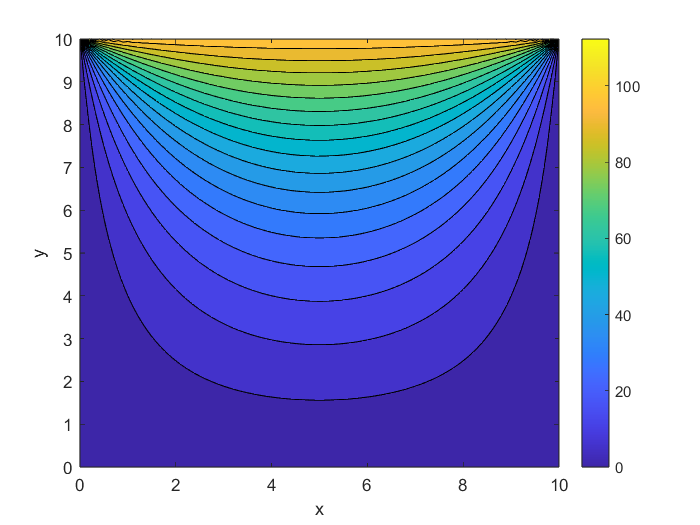
\includegraphics[width=16cm]{fig1.png}
            \caption{第一题结果图} \label{Fig:aa}
        \end{figure}
\end{document}